%--------------------
% Packages
% -------------------
\documentclass[11pt,a4paper,titlepage]{article}
\usepackage[utf8x]{inputenc}
\usepackage[T1]{fontenc}
%\usepackage{gentium}
\usepackage{mathptmx} % Use Times Font


\usepackage[pdftex]{graphicx} % Required for including pictures
\usepackage[english]{babel} % Swedish translations
\usepackage[pdftex,linkcolor=black,pdfborder={0 0 0}]{hyperref} % Format links for pdf
\usepackage{calc} % To reset the counter in the document after title page
\usepackage{enumitem} % Includes lists

\frenchspacing % No double spacing between sentences
\linespread{1.2} % Set linespace
\usepackage[a4paper, lmargin=0.1666\paperwidth, rmargin=0.1666\paperwidth, tmargin=0.1111\paperheight, bmargin=0.1111\paperheight]{geometry} %margins
%\usepackage{parskip}

\usepackage[all]{nowidow} % Tries to remove widows
\usepackage[protrusion=true,expansion=true]{microtype} % Improves typography, load after fontpackage is selected

%-----------------------
% Set pdf information and add title, fill in the fields
%-----------------------
\hypersetup{ 	
pdfsubject = {},
pdftitle = {},
pdfauthor = {}
}

%-----------------------
% Begin document
%-----------------------

\begin{document} %All text i dokumentet hamnar mellan dessa taggar, allt ovanför är formatering av dokumentet
\bibliographystyle{ieeetr}

\begin{titlepage}
  \centering
  \vspace*{2cm}
  {\Huge \textbf{\underline{CS-E4840}}}\\[0.5cm]
  {\Huge \textbf{\underline{\parbox{0.8\linewidth}{\centering Information Visualization D}}}}\\[1.0cm]
  {\Large \textbf{Assignment 2: Basic techniques}} \\
  [1.0cm]
  {\Large Aleksi Kääriäinen (728971)}\\[0.5cm]
  {\Large \today}
\end{titlepage}

\section*{Introduction}
In this assignment, I have completed three visualization tasks using data relating to the SDG selected in assignment 1. Restating just for clarity, I picked SDG number 1, No poverty, for the topic of the assignments.

\section{Visualizing Distributions}
In this task, I identified a variable that is critical for assessing the progress toward the No Poverty SDG. I used the same dataset that was used in assignment 1. The dataset includes data for the share of population living under the poverty line (daily income of US\$30) for most of the countries in the world in the time interval of years 1981-2019. The dataset is publicly available at \cite{data}.

\begin{figure}[h]
    \centering
    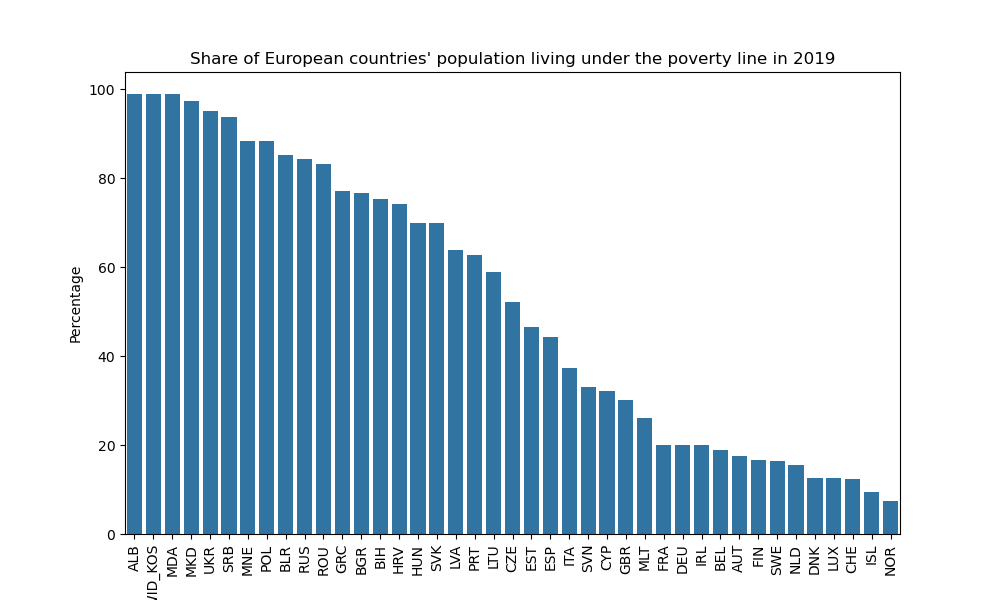
\includegraphics[width=1.0\linewidth]{reports/assignment-2/imgs/assignment2-1.png}
    \caption{Task 1 visualization}
    \label{fig:viz1}
\end{figure}

In figure \ref{fig:viz1}, the distribution of European countries' share of population living under the poverty line in 2019 is visualized. It is a bargraph, where each bar represents a country, and the height of the bar represents the percentage of a given country's population living under the poverty line. In my opinion, the figure is easy to interpret, and fetching statistics for each country is simple. The visualization shows that there is still a lot of work to do to achieve the No Poverty goal of the United Nations 2030 agenda, when there are countries in Europe of whose population almost 100 percent has to fare with a daily income of less than US\$30.

I decided to focus on the wealth distribution of European countries in 2019, since 2019 data is the most recent in the dataset and I wanted to showcase the uneven distribution of wealth in a region that is usually referred to as a single entity. This visualization gives insight to how wealth is distributed within Europe, and even though Europe is generally thought of as a wealthy region, the visualization clearly shows that the wealth is distributed unevenly, and in many countries, the population is very poor.

The dataset was loaded from a csv-file using \texttt{pandas}, and the preprocessing to include only European countries and sorting the data was conducted with the library as well. The plot was created using \texttt{seaborn} and \texttt{matplotlib}'s \texttt{pyplot}. As I am fairly unaccustomed to \texttt{pandas}, I had some troubles getting the data into the wanted form, but after reading the documentation, I was able to overcome the troubles with little effort.

\section{Visualizing Time Series}
In this task, I used the same dataset as in task 1, but this time also utilizing the time dimension of the data. Instead of plotting the distribution for a single year, the distributions have been plotted for each year in the dataset. This visualization, as the one in task 1, focuses on the wealth distribution of European countries.

\begin{figure}[h]
    \centering
    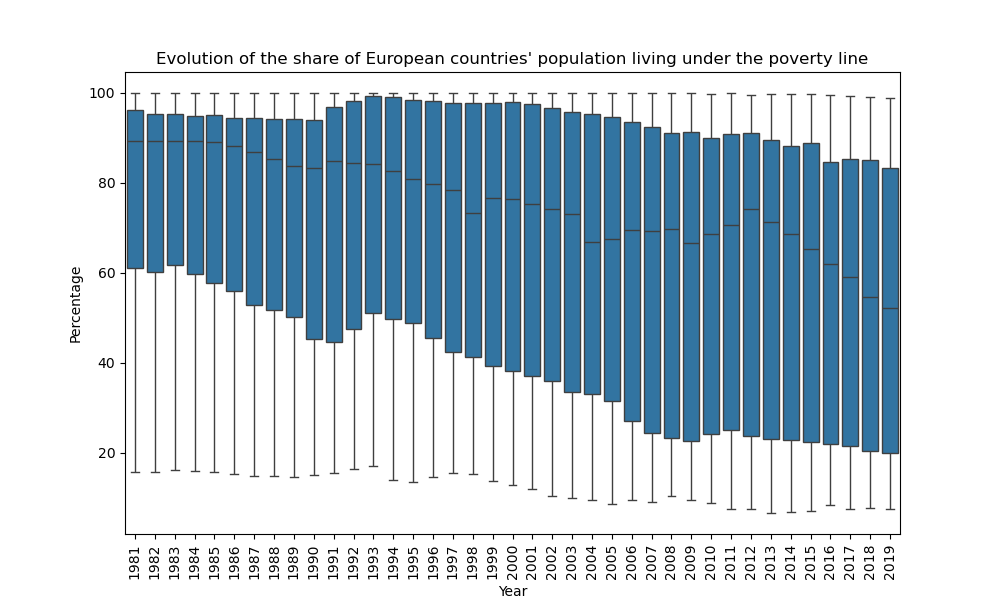
\includegraphics[width=1.0\linewidth]{reports/assignment-2/imgs/assignment2-2.png}
    \caption{Task 2 visualization}
    \label{fig:viz2}
\end{figure}

In figure \ref{fig:viz2}, the distribution of European countries' share of population living under the poverty line is visualized over time as a boxplot. The x-axis shows the year, increasing from left to right, and the y-axis shows the distribution. In each distribution, the orange tick represents the median percentage of all countries. The blue box shows the 25th to 75th percentile distribution, where both parts of the blue box on either side of the median includes 25\% of the distribution. The whiskers extend all the way to the minimum and maximum values, both accounting for 25 percent of the distribution each. The figure clearly shows a trend of decreasing median percentage over time, while also showing some interesting aspects relating to global real-world events. For instance, a small increase in the median in the year 1990 could be due to the 90s depression, and the large bump starting in 2009 is most likely related to the 2009 financial crisis. Even though the median has a decreasing trend, the whiskers of the plot show that the poorest countries have stayed relatively poor during the span of the dataset. The figure also shows that the quartile distributions are increasing in size, meaning that the share of people living under the poverty line is distributed more evenly.

I decided to plot the temporal data as a boxplot, since it is able to show the variance within the distribution as a single plot. Some information, such as single datapoints and which country they represent, are lost when plotting the data as a boxplot, but in my opinion that is permissible, since I wanted to focus more on the distribution, rather than individual datapoints.

I used the same libraries and techniques as in task 1. As such, I had hardly any difficulties making the plot, after having learned the techniques working on task 1. Most of the time spent working on this plot was on deciding which type of plot I wanted to make, and designing the plot itself.

\section{Visualizing High-Dimensional Data}

In the final task of the assignment, high-dimensional data had to be visualized. I used the same dataset for the poverty shares as in task 1 and 2, but in addition to that, I also used a dataset on human development indices published by the United Nations. The dataset is publicly available at \cite{data2}. The dataset lists a number of statistics relating to countries' development in the year 2015. I identified the variables "Life Expectancy at Birth", "Expected Years of Education" and "Gross National Income (GNI) per Capita", as variables that could be related to a country's poverty rate. In order to visualize the data in the way I wanted to, I had to extract the data for the year 2015 from the first dataset, and then join it with the second dataset on the countries' names.

\begin{figure}[h!]
    \centering
    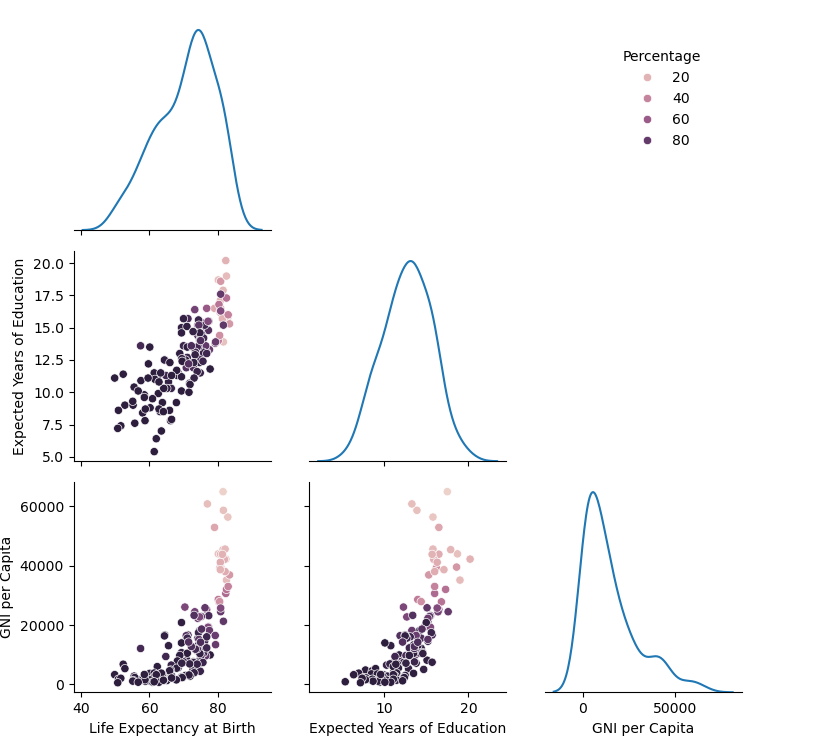
\includegraphics[width=1.0\linewidth]{reports/assignment-2/imgs/task3.png}
    \caption{Task 3 visualization}
    \label{fig:viz3}
\end{figure}

In figure \ref{fig:viz3}, for each country in the dataset, the pairwise relationships between the variables "Life Expectancy at Birth", "Expected Years of Education" and "GNI per Capita" have been plotted as scatterplots. That is to say, each dot on a graph represents a country, with $y = f(x)$ for the variables marked on the axis.  The distributions of the variables are plotted on the diagonal. Additionally, the scatterplots' dots have a colormap added to them. The colormap represents the magnitude of the share of that country's population living under the poverty line. The visualization reveals a clear correlation between the variables, showing that larger numbers in each of the variables result in a smaller poverty share. Rather unsurprisingly though, a country having a large GNI per capita means a lower poverty share without exception.

I thought about which variables to include in the visualization for a long time. All of the variables "Life Expectancy at Birth", "Expected Years of Education" and "GNI per Capita" are among the main statistics used for calculating a country's Human Development Index (HDI). United Nations themselves state, that the HDI "does not reflect on inequalities, poverty, human security, empowerment, etc" \cite{hdi}. I wanted to see, whether there is a relationship between poverty and the HDI statistics by comparing them in this task.

I had some struggles with the data preprocessing and transformations. For example, assigning the percentages to bins was new to me, and joining the two datasets caused some minor headache as well. Again, reading the documentation solved the problems quickly.

\newpage

\bibliography{reports/assignment-2/refs}

\end{document}